\chapter{Tesztelés}
A prototípus tesztelését több lépcsőben zajlott le, minden alkalommal több egységet hozzáadva. Az első a \textbf{hardver} tesztje volt, ahol a \textsl{motorok illesztése}, a \textsl{gearbox}, a \textsl{kamera} és a \textsl{szenzorok} megfelelő működését vizsgáltam, illetve a \textsl{kommunikációt} a Raspberry PI és a PC között. Miután a teszt alapján beállítottam a kamera optimális paramétereit és működésének algoritmusát, a következő teszt a különböző \textbf{célfelismerő algoritmusok} összevetése volt. Itt először egy statikus állványra került a kamera, és a képfelismerés \textsl{sebességét} és \textsl{megbízhatóságát} vizsgáltam. Miután kiválasztódott az optimális megoldás és elkészültek a 3D nyomtatott alkatrészek, kipróbáltam a célfelismerést a motorok mozgásával együtt is. Végezetül pedig \textbf{éles helyzetben} próbáltam ki a prototípust, ami tulajdonképpen céltáblára lövést jelentett. Ekkor vizsgáltam a szerkezet \textsl{stabilitását}, a \textsl{célfelismerést} nagyobb távolságokban, a tüzelési mechanizmus \textsl{megbízhatóságát} és \textsl{pontosságát}, illetve a \textsl{biztonsági funkciókat}.

\section{Elektronikai alkatrészek tesztje}
Ezen teszt során csatlakoztattam a kamerát a Raspberry PI megfelelő csatlakozójához, a NEMA-17 léptetőmotorokat pedig a Stepper Motor HAT csatlakozóihoz. Ezután a GPIO tüskesorhoz csatlakoztattam a lézer diódát, a relé megfelelő lábait, és a végálláskapcsolókat. A gearbox kábeleit összekötöttem a tápegységgel, legvégül pedig a Raspberry PI-t az ethernet porton keresztül a PC-hez csatlakoztattam, majd áram alá helyeztem. Először a Stepper Motor HAT gyártója által szolgáltatott illesztőprogramot próbáltam ki, átkonfigurálva a motor típusának és a microsteppelésnek megfelelően. Ezután a kamera gyári driver-ét teszteltem az \textsl{OpenCV} könyvtár használatával. Végül pedig konfiguráltam a GPIO lábakat, és teszteltem a lézer diódát, a végálláskapcsolókat és a relét. Ezzel együtt teszteltem a kezdetleges szoftvert és az eszközök közötti kommunikációt, ez magába foglalta a \textsl{Socket} és \textsl{Pygame} modulok különböző lehetőségeinek összevetését. A teszt összeállítása a \ref{fig:teszt_1}. ábrán látható. A teszt nem egy alkalommal zajlott le, inkább egy húzódó folyamatként, aminek során megtaláltam az optimális beállításokat a szoftverben.

\begin{figure}[h!]
	\centering
	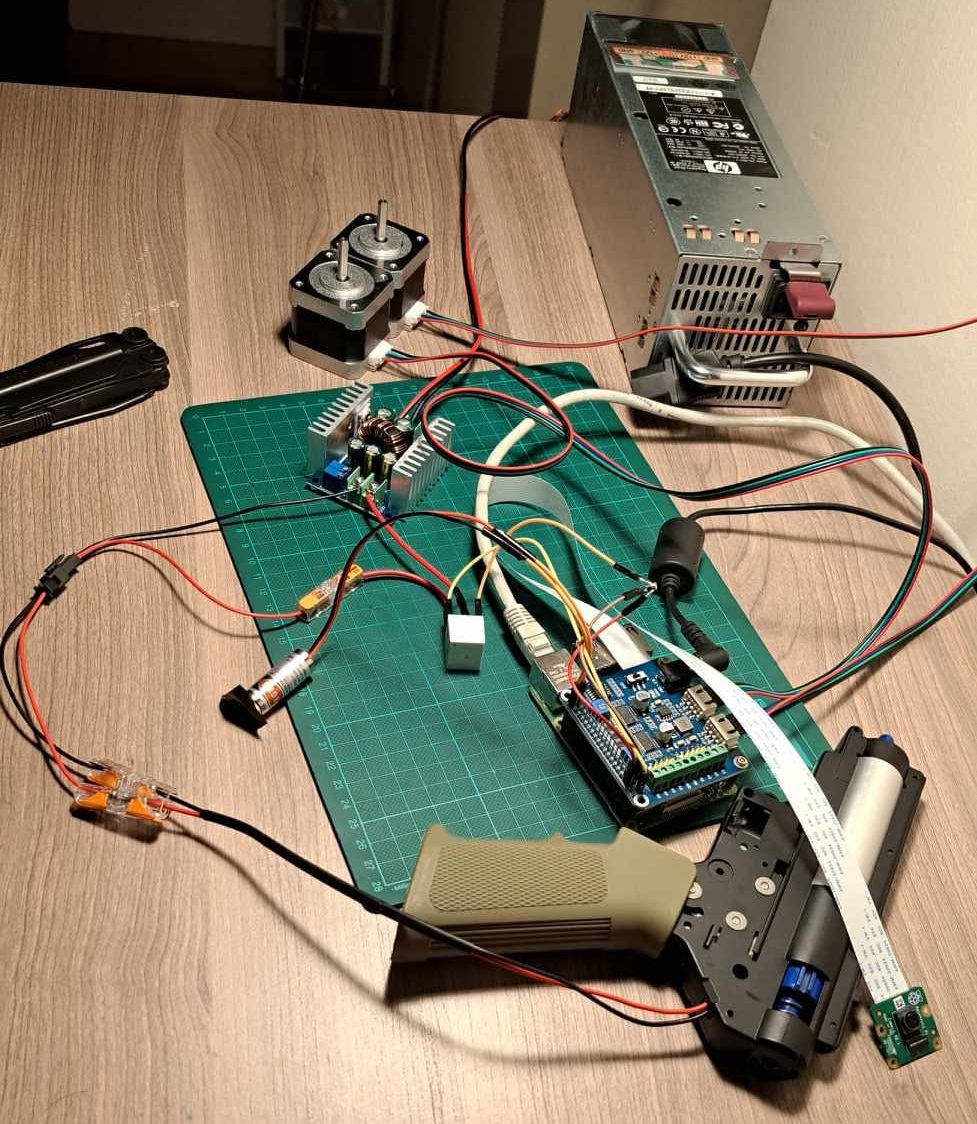
\includegraphics[width=0.5\linewidth]{teszt_1}
	\caption{Elektronikai alkatrészek teszt összeállítása}
	\label{fig:teszt_1}
\end{figure}


\pagebreak


\section{Képfelismerő algoritmusok tesztje}
A teszt összeállítása itt is ugyanaz volt, mint az előző bekezdésben, annyi különbséggel, hogy a kamerát felerősítettem egy állványra. A teszt során a kamera előtt mozgattam az aktuális célpontot, és a célfelismerés megbízhatóságát és sebességét vetettem össze. Először két olyan módszert vizsgáltam, ahol a célpont nem általános, hanem egy PNG képet vesz mintának, és ezt keresi a kamera által szolgáltatott képen, végül pedig egy betanított hálót.

\subsection*{Template Matching}
Erről a módszerről korábban a \ref{sec:soft_template}. bekezdésben volt szó bővebben. A \code{cv2.matchTemplate()} függvény megkeresi a képen a sablont, a \code{cv2.minMaxLoc()} pedig visszaadja a helyzetét, valamint az eredmény pontosságát. Az eredmény pontosságának megszabtam egy alsó határt, és azt változtattam a teszt során. Azt tapasztaltam, hogy ez a módszer nagyon érzékeny a célpont dőlésére és elfordulására, valamint a távolságára is, ezért nem tartottam megfelelő megoldásnak. Emellett minél nagyobb felbontású kép a sablon, a folyamat annál lassabb lesz.
\begin{figure}[h!]
	\centering
	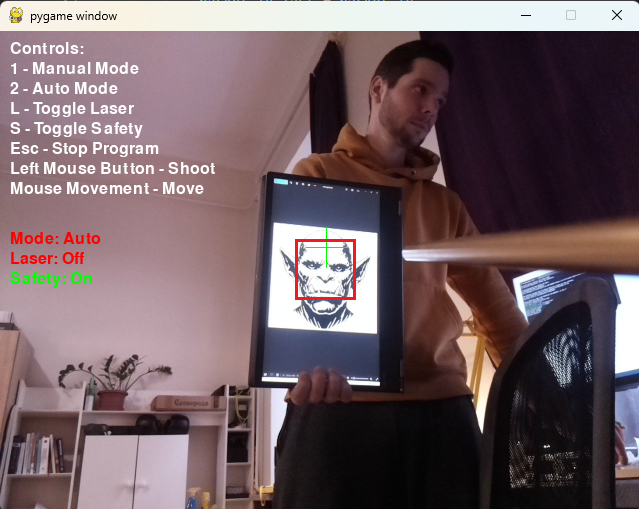
\includegraphics[width=0.8\linewidth]{teszt_auto2}
	\caption{Felismerő algoritmus tesztje}
	\label{fig:teszt_auto2}
\end{figure}
\pagebreak

\subsection*{Feature Matching és Target Tracking}
A feature matching elviekben jól kezeli a célpont torzulását, ezért ezzel kísérleteztem a későbbiekben. Az elképzelés az volt, hogy a feature matching megtalálja megbízhatóan a célpontot, majd a target tracking képes lesz gyorsan követni. A gyakorlatban, amennyiben egyszer megtalálta az algoritmus a célpontot, onnan tényleg pontosan tudta követni, azonban magával a felismeréssel voltak itt is a problémák. Nagyon megbízhatatlan volt, ha az érzékenységet lentebb állítottam, akkor fals pozitívot is mutatott, ha fentebb, akkor pedig nem találta meg a célpontot. A target tracking is csak akkor működött, ha a kamera egy helyben maradt. Ha már a motorok is mozogtak, akkor könnyedén elvesztette a célpontot.

\subsection*{Haar Cascade}
Az utolsó módszer, amit teszteltem, az a Haar Cascade és tanított neurális hálók használata volt. Ez az előzőekhez képest meglepően megbízható volt, a célpontot felismerte viszonylag távolról is, akár rossz fényviszonyok között is. A célpont kb 15 fokos dőlése esetén szintén felismerte azt, amit én megfelelőnek találtam. Ezzel a módszerrel folytattam a munkát. \\

Miután eldöntöttem, melyik módszerrel haladok tovább, kipróbáltam az algoritmust a fegyver mozgásával összhangban. Ennek módja az volt, hogy a kamera előtt, egy laptopon mozgattam a sablon. Erről kép látható a \ref{fig:teszt_auto2}. ábrán.

\pagebreak

\begin{figure}[h!]
	\centering
	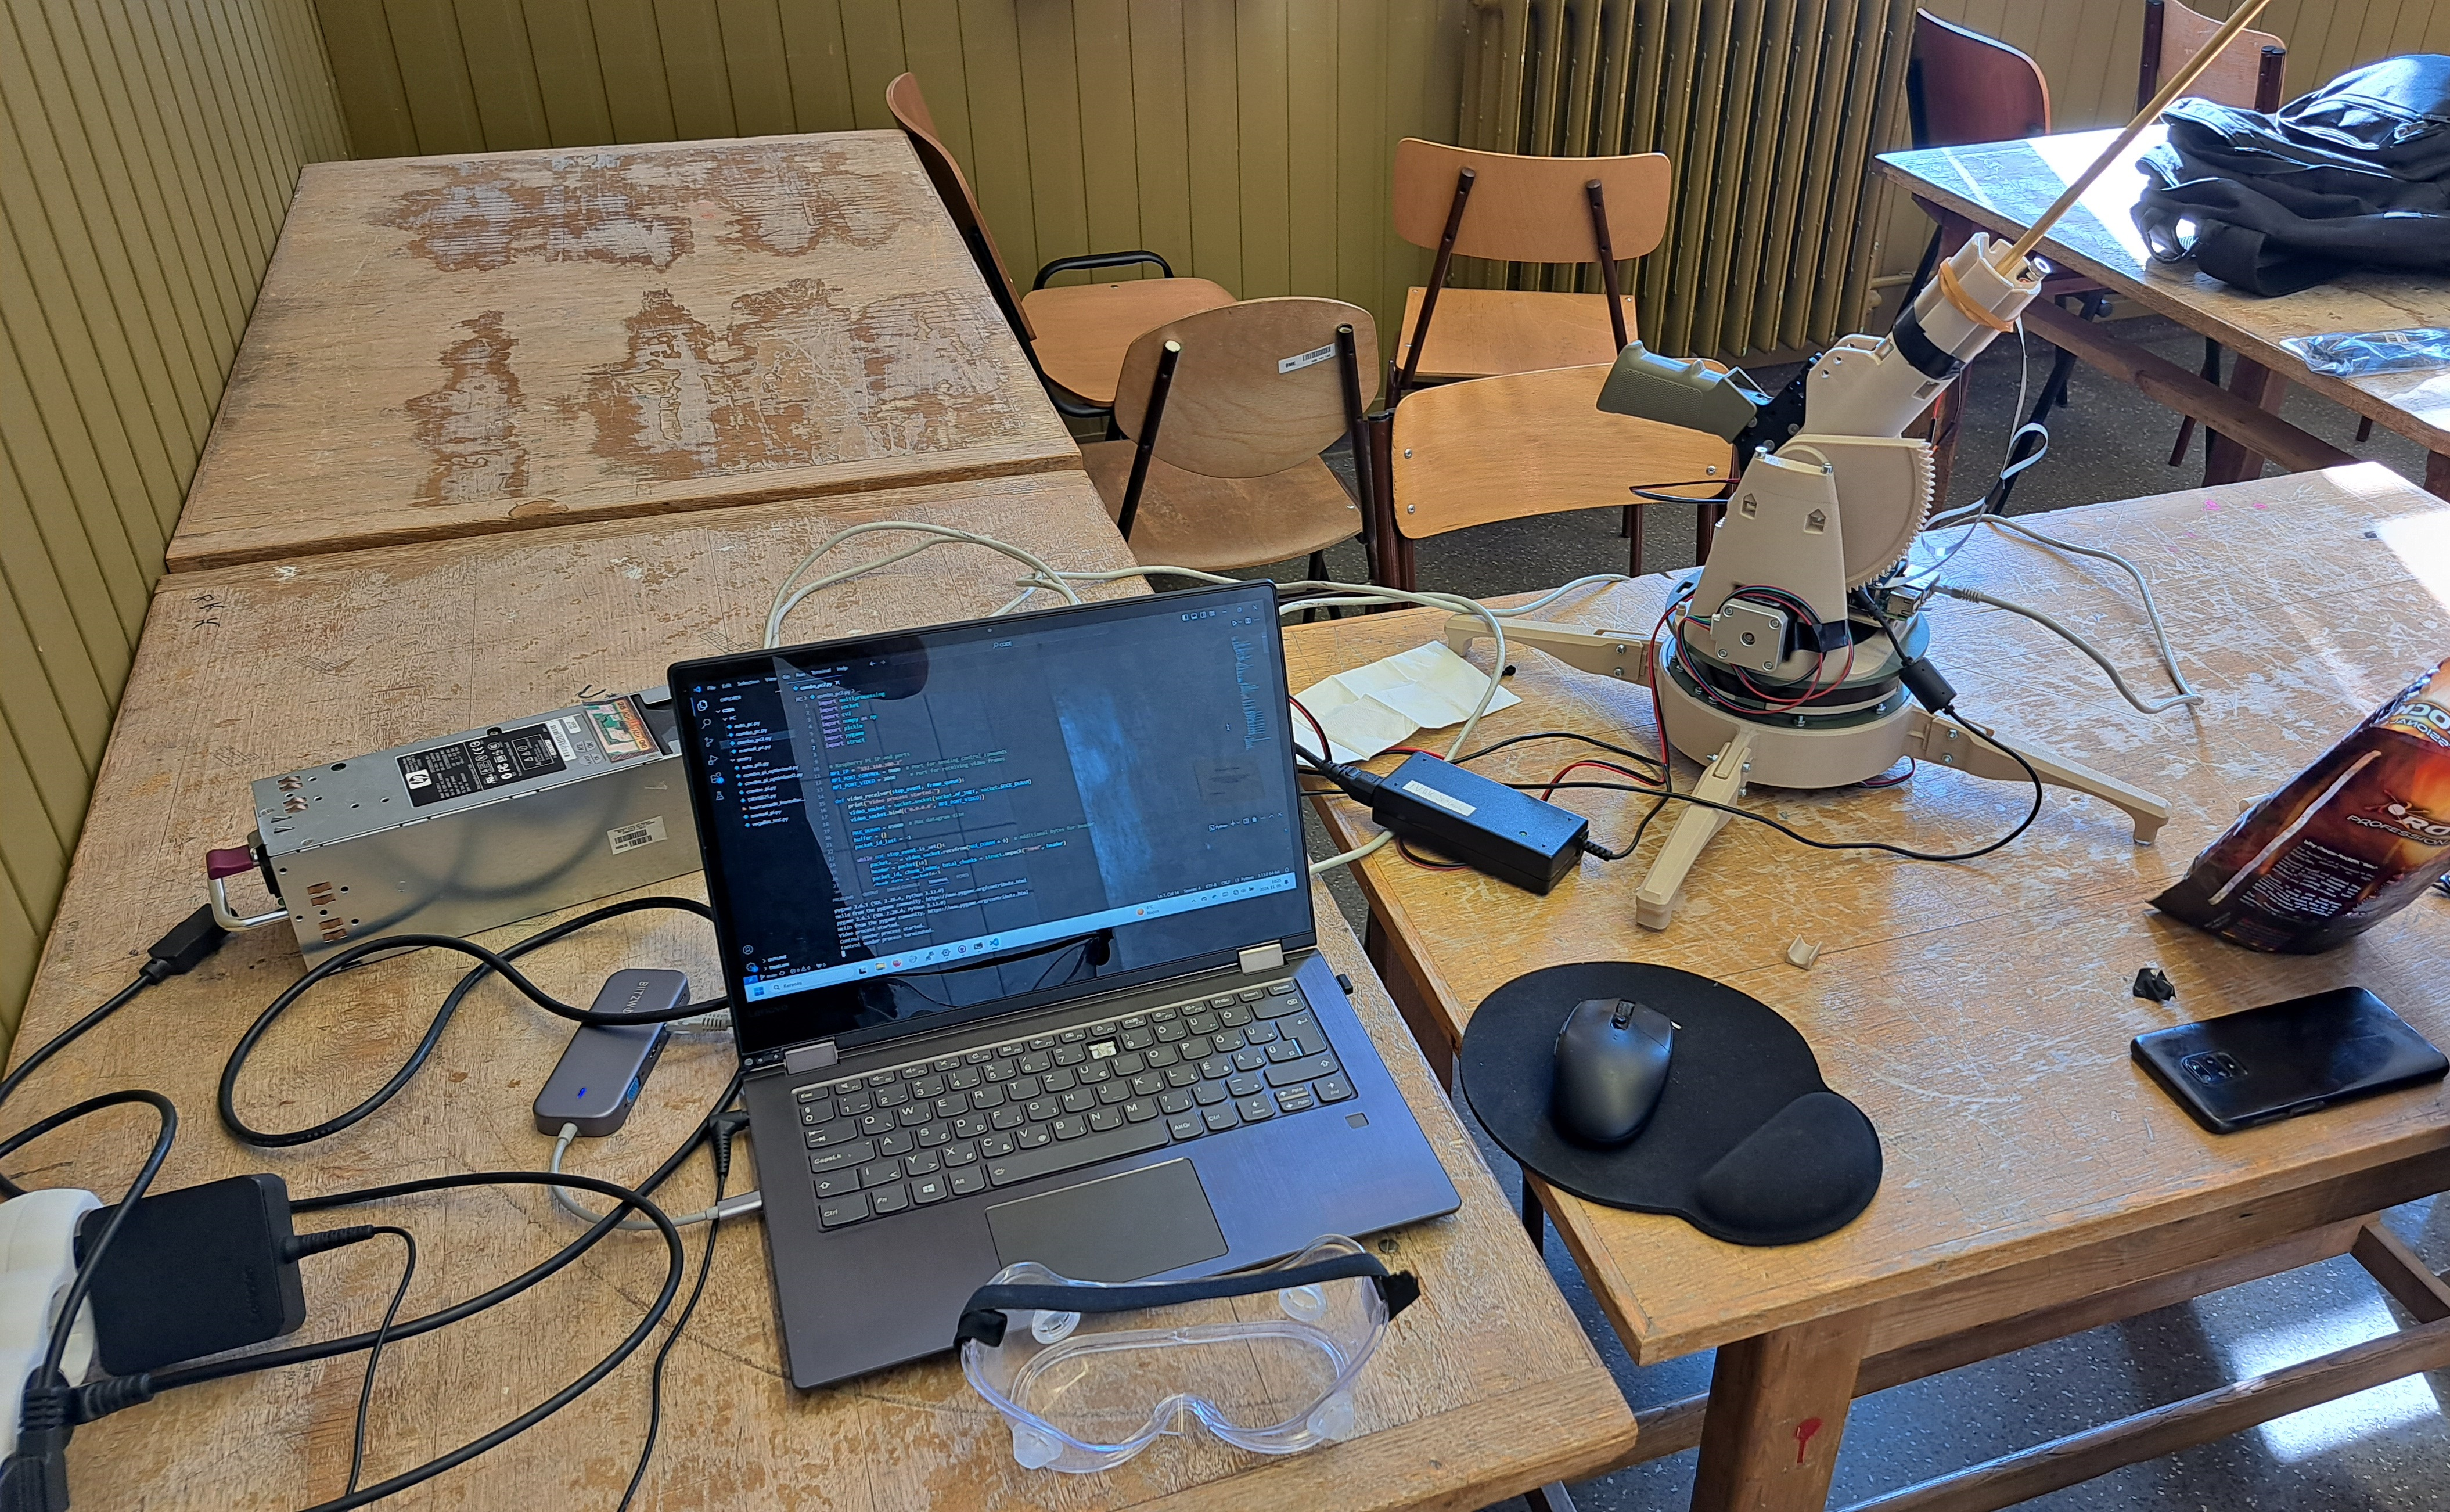
\includegraphics[width=1\linewidth]{teszt_setup2}
	\caption{Az éles teszt környezete}
	\label{fig:teszt_teszt_setup1}
\end{figure}

\begin{figure}[h!]
	\centering
	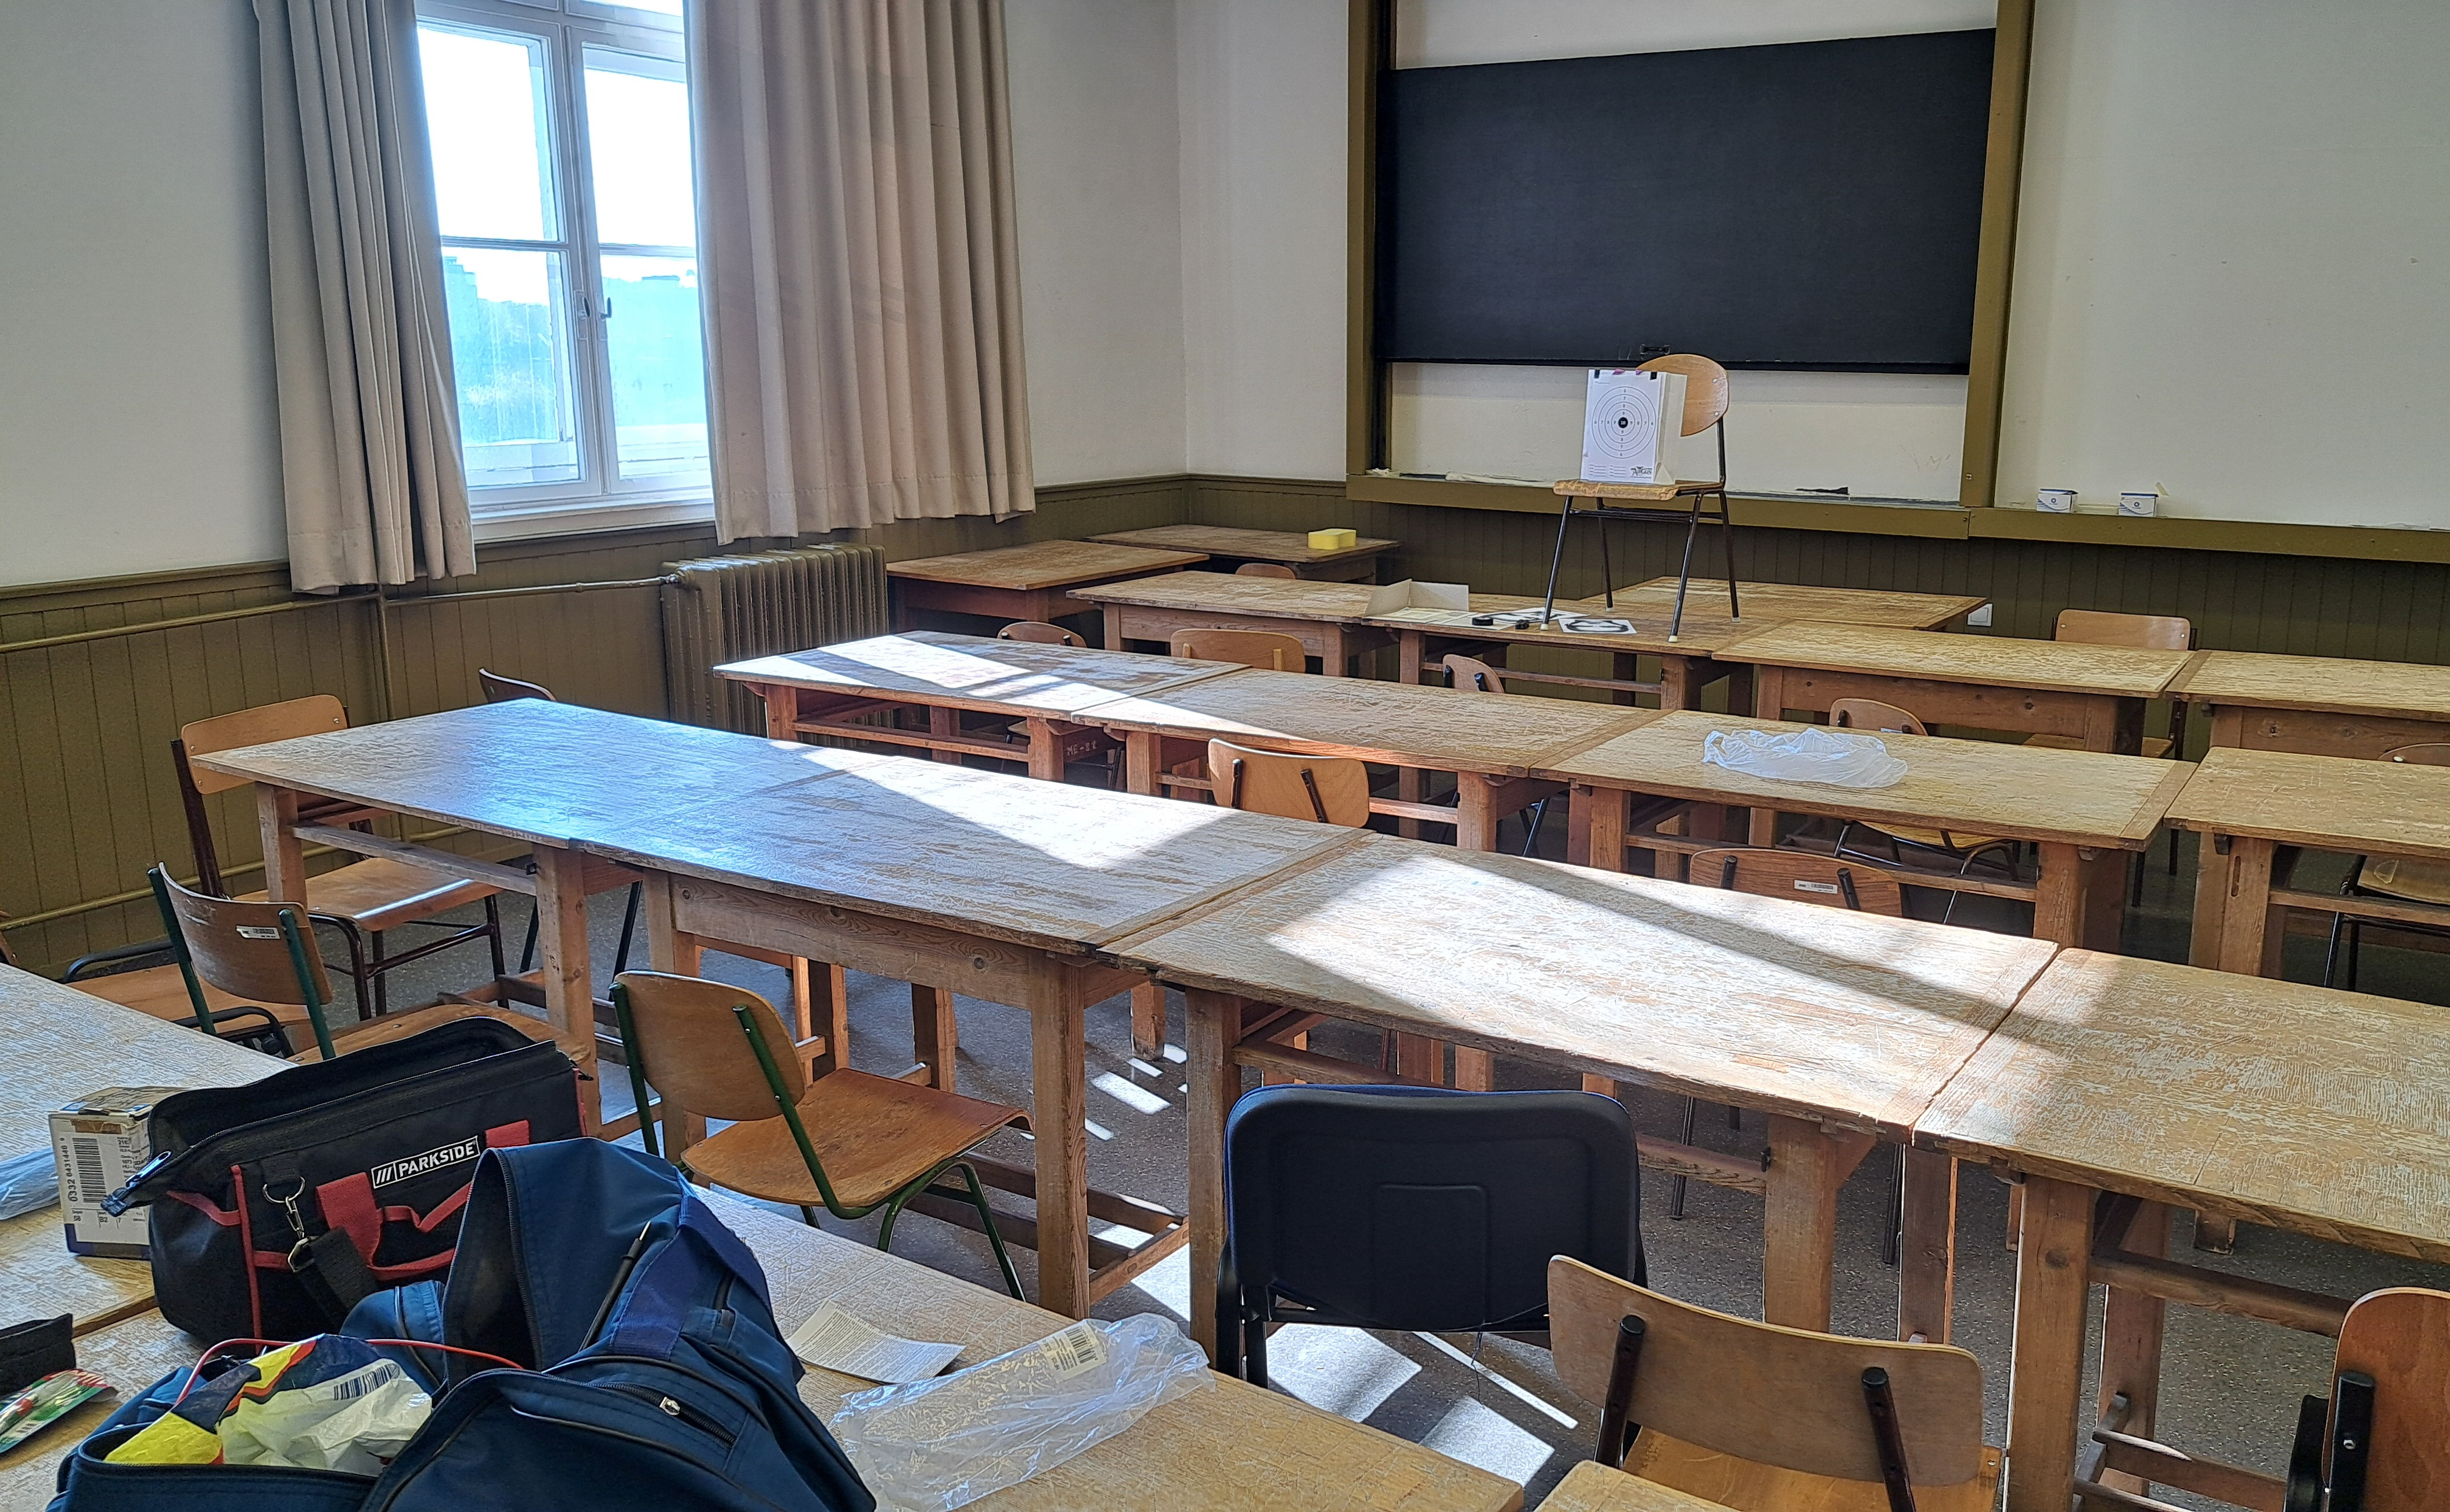
\includegraphics[width=1\linewidth]{teszt_setup1}
	\caption{Az éles teszt környezete}
	\label{fig:teszt_teszt_setup2}
\end{figure}

\pagebreak

\section{Éles teszt}
A tesztet egy jól megvilágított tanteremben végeztem. Az eszköz egy stabil padon állt, a célpont pedig 5 méterrel előtte, és kb. fél méterrel fölötte. A célpont a \ref{fig:teszt_teszt_setup2}. ábrán látható.\\

A teszt során a manuális működési móddal kezdtem, azon belül a fegyver kalibrálásával. Először azt tapasztaltam, hogy a kamera képének a közepe nem ott van, ahova a fegyver csöve mutat. Ezért a célkeresztet addig mozgattam a képen, amíg oda nem mutatott, ahova a fegyver ténylegesen lőtt. Ezután a rendszer nagy pontossággal tudott lőni, tulajdonképpen az összes leadott lövés a hibahatáron belül volt. A lézer irányzékot azonban nem tudtam pontosan beállítani, 5 méteren nagyjából 10-15 cm-t téved. A következő ábrákon látható a teszt eredménye. 5-ös sorozatokban tüzeltem, mindig a cél közepére irányítva a kamera célkeresztjét. \\

A következő teszt az arcfelismerés, és a követés funkció tesztje volt. A körülmények ugyanazok maradtak, és szintén 5 m-re volt a célpont. A teszt során egy kolléga tartotta a kinyomtatott arcképet, és mozgatta, változtatva a sebességet és irányt. Természetesen a gearbox nem volt áram alatt, és a kolléga is viselt védőszemüveget. Azt tapasztaltam, hogy a fegyver körülbelül a sétáló ember sebességét tudja követni 5 m távolságban, és igen pontosan be tudja célozni. A tesztkörnyezet a \ref{fig:teszt_teszt_setup1}. és \ref{fig:teszt_teszt_setup2}. ábrákon látható.

Összességében elmondható, hogy a beállított célkereszttel, 5 méterről igen pontos eredmények születtek. 4 leadott sorozat során 5-5 golyót lőttem ki, az eredmények az alábbi ábrán láthatóak:

\begin{figure}[h!]
	\centering
	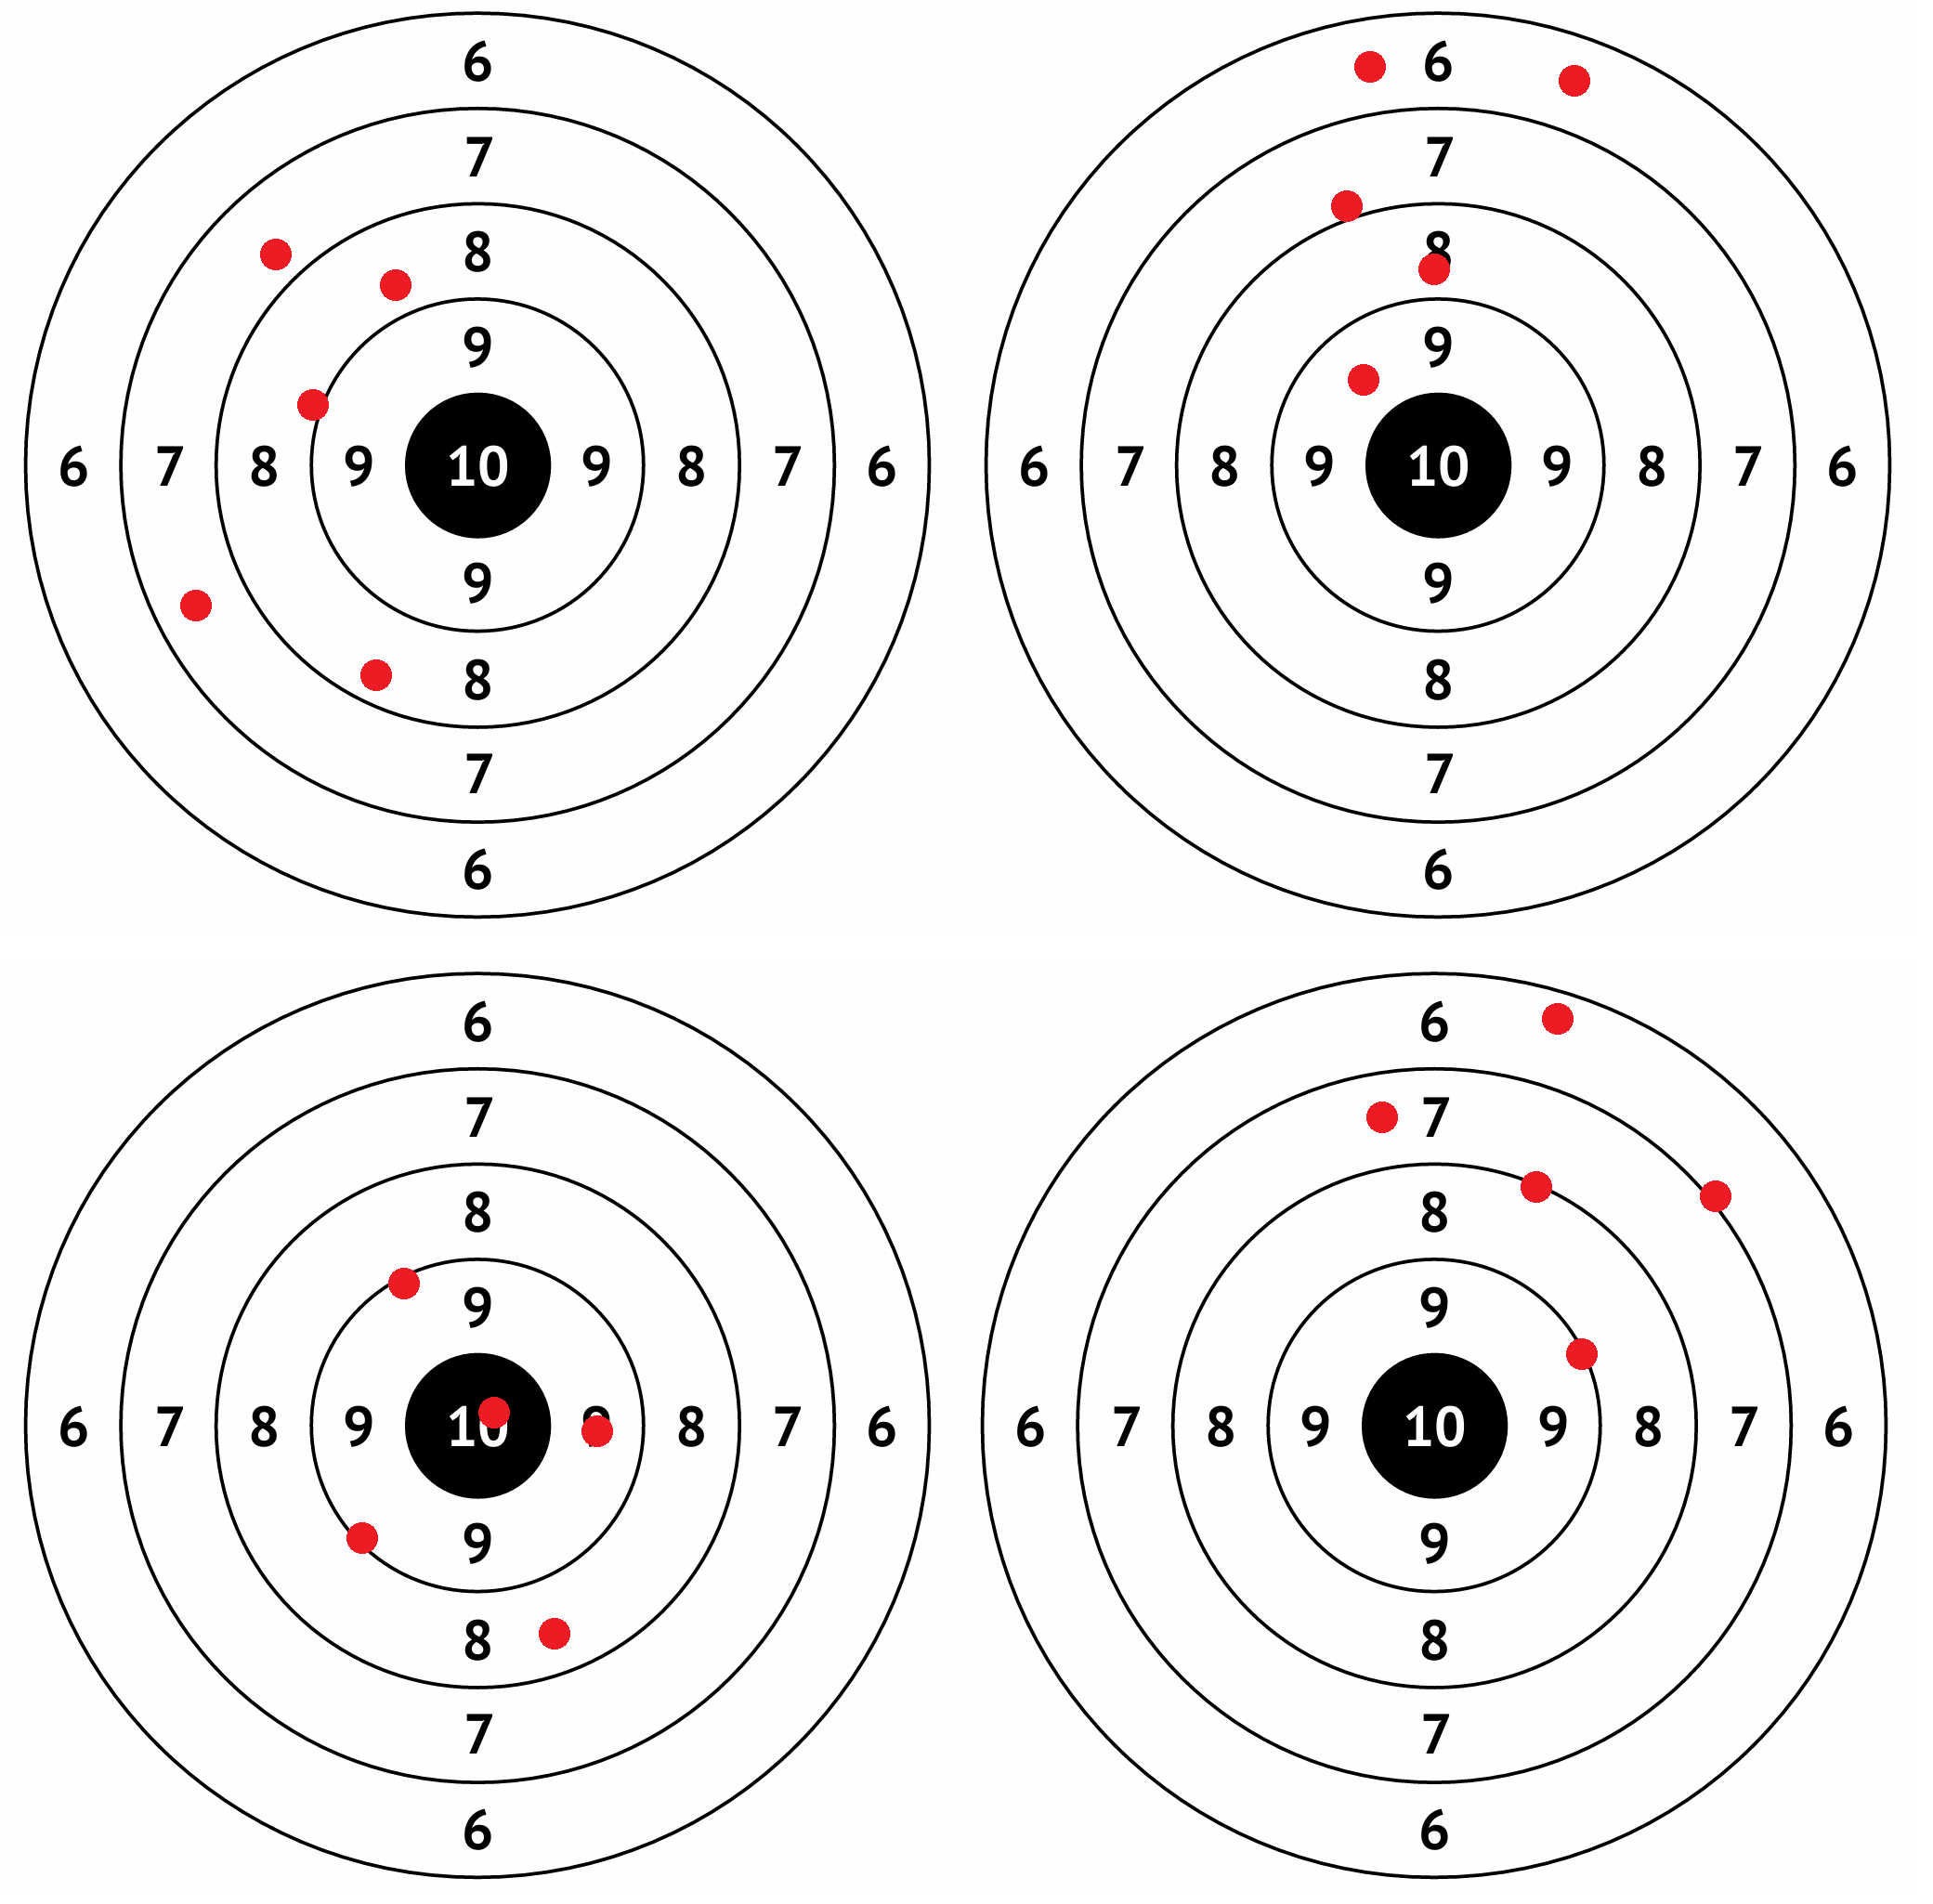
\includegraphics[width=0.6\linewidth]{teszt_eredmenyek}
	\caption{Az éles teszt eredményei}
	\label{fig:teszt_eredmenyek}
\end{figure}